\chapter{Propuesta Metodológica}

En este capítulo vamos a definir y a detallar los procesos que vamos a seguir para llevar a cabo la propuesta pedagógica definida en el capítulo anterior.

\section{Herramientas necesarias}

\subsection{Sistemas de control de versiones}

Lo primero que necesitaremos es enseñar a nuestros alumnos a utilizar un sistema de control de versiones, aunque existen varios sistemas (SVN, Mercurial, CVS), hoy en día estándar de facto es Git que además es software libre.

Para una administración más sencilla de nuestro código utilizaremos un cliente web como es GitHub, aunque existen otros como pueden ser GitLab o BitBucket.

\subsubsection {Git}

Git es un sistema de control de versiones distribuido para el seguimiento de los cambios en el código fuente durante el desarrollo de software. Está diseñado para coordinar el trabajo entre programadores, pero se puede utilizar para realizar un seguimiento de los cambios en cualquier conjunto de archivos.  Sus objetivos incluyen la velocidad, la integridad de los datos y la compatibilidad con flujos de trabajo distribuidos y no lineales.

Git fue creado por Linus Torvalds en 2005 para el desarrollo del núcleo de Linux.

Como con la mayoría de los sistemas de control de versiones distribuidos, y a diferencia de la mayoría de los sistemas cliente-servidor cada directorio de Git es un repositorio completo con un historial completo y capacidades de seguimiento de versiones completas, independiente del acceso a la red o a un servidor central.

Git es software libre y de código abierto distribuido bajo los términos de la Licencia Pública General GNU versión 2.

\subsubsection {GitHub}

GitHub es un servicio de alojamiento basado en web para el control de versiones a través de Git, fue adquirido por MicroSoft en 2018. Se utiliza sobre todo para código fuente. Ofrece toda la funcionalidad de control de versiones distribuido y gestión de código fuente de Git, además de añadir sus propias características.

Proporciona control de acceso y varias funciones de colaboración como seguimiento de errores, pull requests, gestión de tareas y wikis para cada proyecto. Además cuenta con un sub-proyecto llamado GitHub Education que es ampliamente utilizado como herramientas para la formación de programadores (\cite{hernandez_integracion_2018}).


\section {Sistemas de integración continua (CI)}

\subsubsection {Travis-CI}

Travis CI es un servicio alojado de integración continua que se utiliza para construir y testear proyectos de software alojados en GitHub.

Los proyectos de código abierto pueden ser probados de forma gratuita a través del sitio travis-ci.org. En cambio los proyectos privados deben pagar para poder ser ejecutados a través del sitio travis-ci.com.

Gran parte del código fuente de Travis CI es software libre y está disponible en GitHub.

\subsection{Lenguajes utilizados}

Al igual que no existe una única solución a un problema, existen multitud de lenguajes de programación, nosotros nos vamos a centrar en solamente cuatro de ellos y vamos a explicar los motivos:

\subsubsection{Python}

Python es un lenguaje de programación interpretado cuya filosofía hace hincapié en una sintaxis que favorezca un código legible. Fue desarrollado por Guido van Rossum en 1991 y hoy en día es uno de los lenguajes de programación más utilizados en cursos de introducción a la programación ya que su sintaxis suele ser más sencilla, asemejándose al ``pseudocódigo''.

Según el (REFERNCIA A ESTUDIO STACKOVERFLOW) Python es uno de los lenguajes con mayor proyección de futuro y que del que mas se ha incrementado su uso, además (REFERENCIA A DJANGO-GIRLS), referencia a estudios

Basándonos en las recomendaciones del Python Consortium (REFERENCIA A LA RECOMENDACIÓN DE LA PYTHON CONSORTIUM) vamos a centrar nuestros ejercicios en Python3 ya que no tiene sentido enseñar a nuestros alumnos Python2 pues además de desaconsejado, este lenguaje va a perder su soporte en un futuro muy cercano (REFERENCIA AL FIN DE SOPORTE DE PYTHON2).

\subsubsection{Ruby}

Ruby es un lenguaje de programación creado por el programador japonés Yukihiro Matsumoto en 1995. Es un lenguaje fuertemente orientado objetos ya que todos los tipos de dato son a su vez un objeto.

\bigskip
Ruby empezó a ganar popularidad tras la publicación del framework de aplicaciones web Ruby On Rails (RoR) por parte de David Heinemeier Hansson en 2005 ya que el mismo simplificaba muchísimo el desarrollo siguiendo el patrón Modelo Vista Controlador (MVC).

\bigskip
Debido a su sencilla sintaxis y su fuerte orientación a objetos es ampliamente utilizado para enseñar las particularidades de dicho paradigma.

\subsubsection{C}

El lenguaje de programación C es un lenguaje de propósito general desarrollado por Dennis Ritchie en los Laboratorios Bell entre 1969 y 1972, es el lenguaje de programación más popular para crear software para sistemas embebidos y micro-controladores, aunque también se puede utilizar para crear aplicaciones.

\bigskip
Es un lenguaje tipado estáticamente (en tiempo de compilación) y considerad de de medio nivel ya que dispone de las estructuras típicas de los lenguajes de alto nivel pero permitiendo un control a muy bajo nivel. Los compiladores suelen ofrecer extensiones al lenguaje que posibilitan mezclar código en ensamblador con código C, acceder a memoria o controlar diferentes dispositivos.

\subsubsection{HTML}

El lenguaje de marcas de hipertexto o HTML por sus siglas en inglés, es un lenguaje de marcado para la elaboración de páginas web. La primera versión del lenguaje fue creada por Tim Berners-Lee en 1991 mientras trabajaba en el Centro Europeo de Investigaciones Nucleares (CERN) en Suiza. Actualmente sus especificaciones están a cargo del World Wide Web Consortium (W3C).

\bigskip
HTML no es un lenguaje de programación, es un lenguaje de marcado que sirve para definir documentos estandarizados.


\section {Herramientas de validacion de código}

Son conocidos como ``linters'' y

\subsection{rubocop}

Tiene opciones interesantes como validar la complejidad ciclomática\footnote{Valor escalar que mide la complejidad lógica de un programa.}

\section {Herramientas de verificación de código}

Las herramientas de verificación de código se utilizan para verificar que el código está bien escrito, pueden comprobar la sintaxis, el estilo o ambas cosas. Pasamos a enumerar las más comunes:

\subsection {Pytest}

Pytest es un framework de test unitarios para el lenguaje de programación Python que facilita la creación de pruebas sencillas y escalables. Las pruebas son expresivas y legibles y no se requiere código adicional.

\subsection {PEP8}

PEP8 es una guía de estilo de codificación para Python definida por sus creadores y que está definida como el estilo estándar del lenguaje.

\subsection {RSpec}

RSpec es una herramienta para realizar test BDD que sirve para probar código escrito en el lenguaje de programación Ruby. Se utiliza ampliamente en aplicaciones de producción.

\subsection {Tidy}

HTML Tidy es una aplicación de consola que sirve para corregir código HTML no válido, detectar posibles errores de accesibilidad web y mejorar el diseño y el estilo de sangría del marcado resultante. Fue desarrollado en 2002 por Dave Raggett, miembro del World Wide Web Consortium (W3C).

\section{Metodología de aprendizaje}

Algunas de las herramientas necesarias para nuestro sistema de corrección requieren algo de formación previa, por lo que vamos a definir una metodología de aprendizaje para las mismas

\subsection{Aprendiendo a usar Git}

Como ya explicamos anteriormente Git es uno de los sistemas de control de versiones más utilizados en la actualidad. Es dificil encontrar hoy en día una empresa que se dedique a la programación de forma profesional que no la utilice. A pesar de ello no forma parte del currículo de los ciclos formativos de informática. De hecho, salvo contadas excepciones, tampoco se aprende su uso en los Grados en Ingeniería Informática. De ahí la ventaja de nuestro sistema, ya que vamos a aprovechar para enseñarles a utilizar una herramienta que van a usar de forma exhaustiva durante su futura carrera profesional.

\bigskip
Para aprender a utilizar Git nos vamos a basar en diversos manuales que enseñan a utilizarlo de una forma sencilla (\cite{popov_control_2012}) sin necesidad de tener conocimientos de programación.

\subsubsection{Introducción a Git}

Un sistema de control de versiones es una herramienta que registra los cambios realizados sobre un conjunto de archivos a lo largo del tiempo, de modo que se pueden volver a un estado previo en cualquier momento. Aunque se usa de forma mayoritaria para código fuente  se pueden guardar versiones de cualquier tipo de archivo.

\bigskip
Las principales características de un sistema de control de versiones son revertir archivos a un estado previo, revertir el proyecto entero a un estado anterior, comparar cambios a lo largo del tiempo, ver quién modificó por última vez algo que puede estar causando un problema así como saber quién introdujo un error y cuándo.

\bigskip
Un método de control de versiones usado por mucha gente es copiar los archivos a otro directorio (indicando la fecha y hora en que lo hicieron, si son avispados). Este enfoque es muy común porque es muy simple, pero también tremendamente propenso a errores. Es fácil olvidar en qué directorio te encuentras, y guardar accidentalmente en el archivo equivocado o sobrescribir archivos que no querías.

\bigskip
En cambio Git es un sistema de control de versiones distribuido, los clientes no sólo descargan la última instantánea de los archivos: replican completamente el repositorio. Así, si un servidor muere, y estos sistemas estaban colaborando a través de él, cualquiera de los repositorios de los clientes puede copiarse en el servidor para restaurarlo (figura \ref{fig:dvcs}).

\begin{figure}[H]
\centering
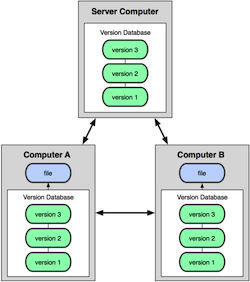
\includegraphics{../images/dvcs}
\caption{Diagrama de control de versiones distribuido}
\label{fig:dvcs}
\end{figure}

\subsubsection{Creando una cuenta en GitHub}

Para crear una cuenta en GitHUb debemos acceder a su página web \url{https://github.com} y hacer clic en SignUp (figura \ref{fig:git1}).

\begin{figure}[H]
\centering
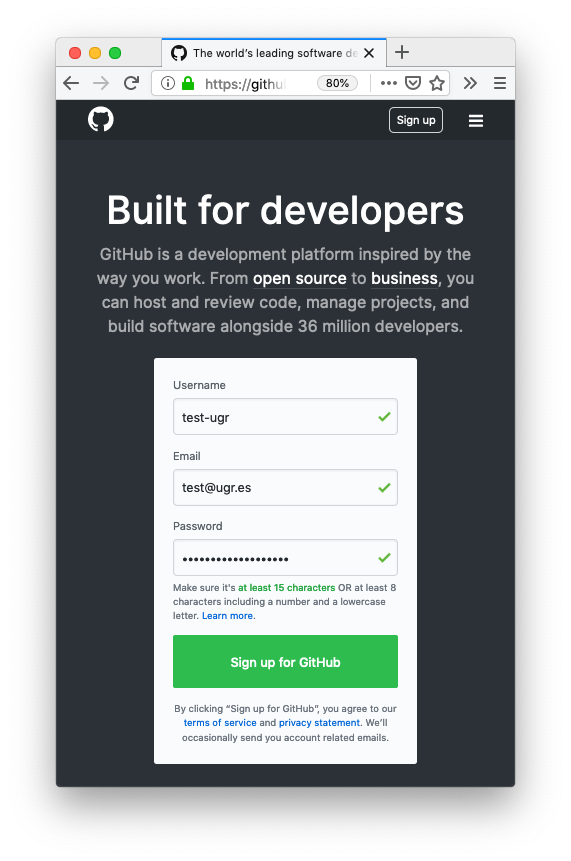
\includegraphics[width=1.0\textwidth]{../images/git1}
\caption{Pagina de registro de GitHub}
\label{fig:git1}
\end{figure}

\subsubsection{Creando nuestro primer repositorio}

Crear un repositorio en GitHub es muy intuitivo, solo tenemos que hacer clic en el botón New y rellenar los datos que nos solicita (figura \ref{fig:git2}). De igual forma podemos crear un repositorio de forma local en nuestro ordenador ejecutando el comando \texttt{git init}

\begin{figure}[H]
\centering
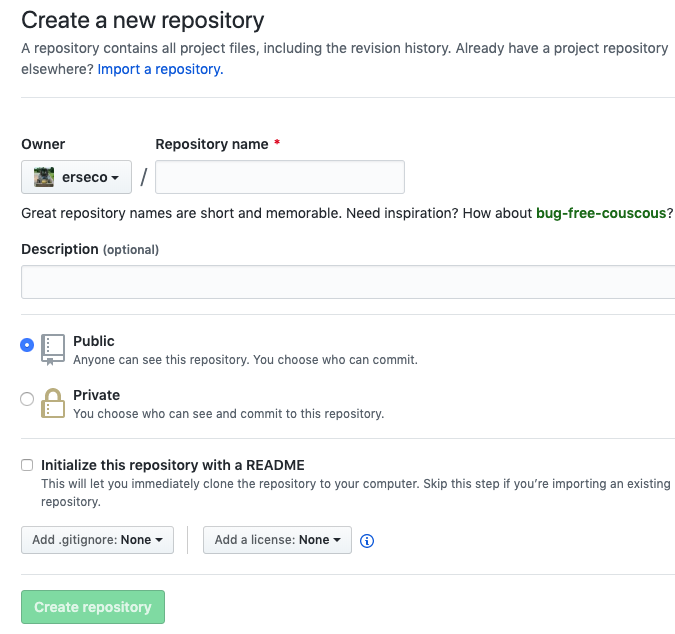
\includegraphics[width=1.0\textwidth]{../images/git2}
\caption{Ventana de creación de repositorio en GitHub}
\label{fig:git2}
\end{figure}

\subsubsection{Comandos básicos de Git}

Aquí podemos ver algunos de los comandos más habituales de Git, se puede encontrar la referencia completa en su documentación oficial en \url{https://git-scm.com/doc}.

\begin{itemize}
  \item \textbf{git clone}: Clona un repositorio
  \item \textbf{git status}: Nos dice el estado de un repositorio
  \item \textbf{git commit}: Nos permite guardar los cambios en una rama
  \item \textbf{git checkout}: Nos permite cambiar de rama
  \item \textbf{git branch}: Nos permite crear y listar ramas
  \item \textbf{git push}: Permite enviar el código a un repositorio remoto
  \item \textbf{git pull}: Permite obtener el código desde un repositorio remoto
\end{itemize}


\subsubsection{Creando nuestro primer Fork}

Una bifurcación, o fork en inglés, es el término que se utiliza para indicar una ramificación de un trabajo. Básicamente significa que vamos a copiar un proyecto y crear uno nuevo haciéndole modificaciones. La capacidad de crear bifurcaciones de código de forma sencilla es una de las características que han ayudado a la plataforma GitHub llegar a ser el sitio de referencia para albergar proyectos de software libre.

\bigskip
Para crear un fork en GitHub de cualquier proyecto simplemente tenemos que hacer click en el botón situado a la derecha de cada proyecto (figura \ref{fig:git_fork}). Una cosa a tener en cuenta a la hora de hacer un Fork de un proyecto es la licencia bajo la que esté dicho código, el cual suele venir indicado en el fichero LICENSE, no todas las licencias permiten la libre distribución de proyectos derivados.

\begin{figure}[H]
\centering
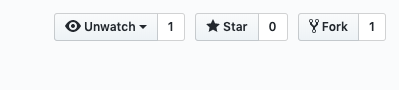
\includegraphics[width=1.0\textwidth]{../images/git_fork}
\caption{Detalle del botón de Fork en GitHub}
\label{fig:git_fork}
\end{figure}

\subsubsection{Creando un Pull-Request}

Las contribuciones a un repositorio de código fuente que utiliza un sistema de control de versiones distribuido se realizan comúnmente por medio de un ``pull request''. El colaborador solicita que el encargado del proyecto haga un ``pull'' con los cambios en el código fuente, de ahí el nombre. El mantenedor puede revisar el conjunto de cambios, discutir modificaciones potenciales o mezclar el código.

Dependiendo del flujo de trabajo establecido el código puede ser probado antes de ser incluido en la versión oficial. Algunos proyectos ejecutan un conjunto de pruebas automatizadas en cada solicitud de extracción, utilizando una herramienta de integración continua como Travis CI, y el revisor verifica que cualquier código nuevo tenga la cobertura de pruebas adecuada.

Para hacer un ``Pull request'' haremos clic en el botón ``New pull request'' y seleccionando que ramas queremos fusionar (figura \ref{fig:git_pr}).

\begin{figure}[H]
\centering
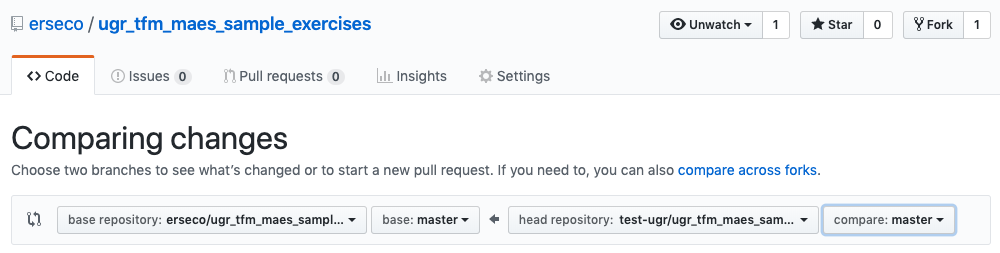
\includegraphics[width=1.0\textwidth]{../images/git_pr}
\caption{Detalle de creación de un Pull Request en GitHub}
\label{fig:git_pr}
\end{figure}


\subsubsection{Sistemas de integración continua (CI)}

Un sistema de integración continua suele consistir en una plataforma que ejecuta una serie de pasos con cada ``Push'' que realizamos a nuestro sistema de control de versiones. A esta serie de pasos se le suele denominar ``pipeline'' y suele contener pasos habituales como pueden ser la compilación, la ejecución de validaciones sintácticas y estilísticas de código (\textit{linter}) y la ejecución de los diferentes test para comprobar que efectivamente el código funciona.

\bigskip
Como ya hemos indicado, para nuestra metodología vamos a utilizar ``Travis CI'' aunque la forma de funcionar es muy similar en casi todas las plataformas. Para crear una cuenta en ``Travis CI'' iremos a la url \url{https://travis-ci.org} y haremos click en el botón ``Sign-Up'' (figura \ref{fig:travis_signup})).

\begin{figure}[H]
\centering
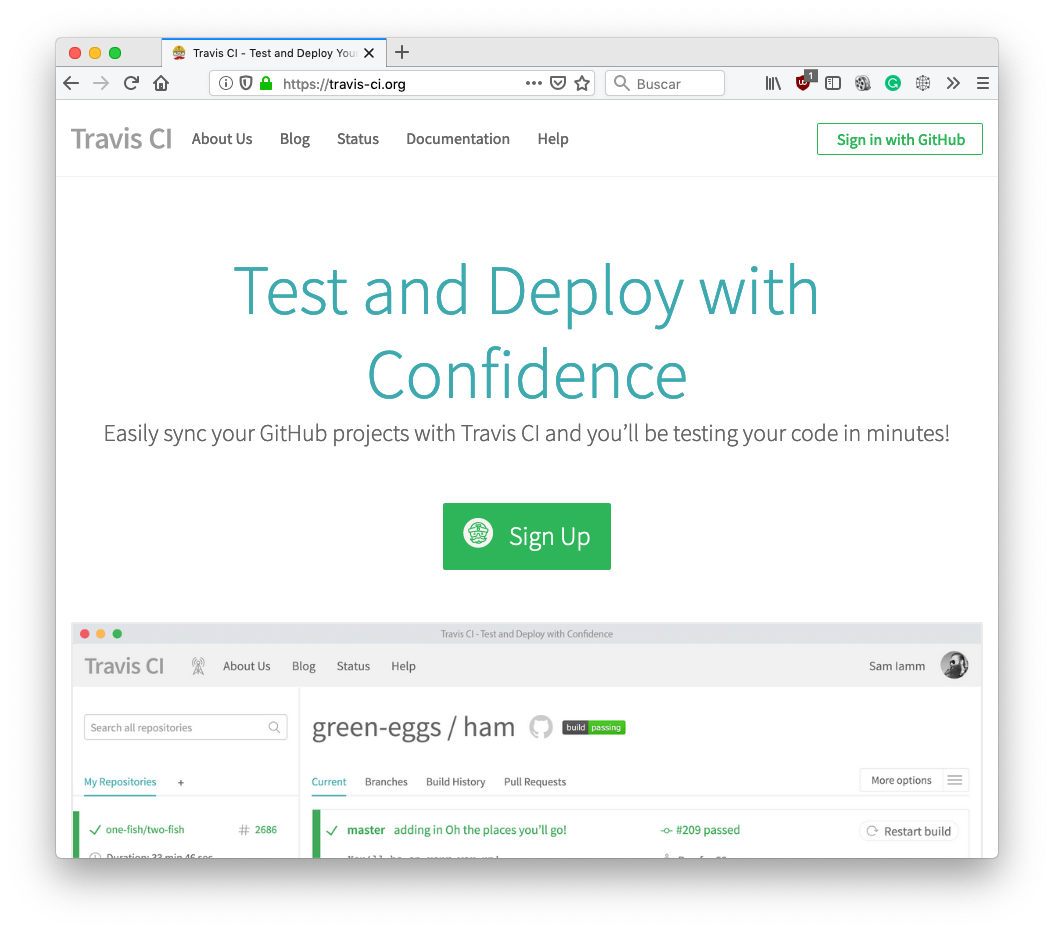
\includegraphics[width=1.0\textwidth]{../images/travis_signup}
\caption{Detalle de creación de una cuenta en Travis CI}
\label{fig:travis_signup}
\end{figure}

Una vez tengamos nuestra cuenta tenemos que activar en cuales de nuestra lista de repositorios queremos activar el servicio. Para ellos solo debemos hacer click en el interruptor hasta que quede de color verde (figura \ref{fig:travis_enable}).

\begin{figure}[H]
\centering
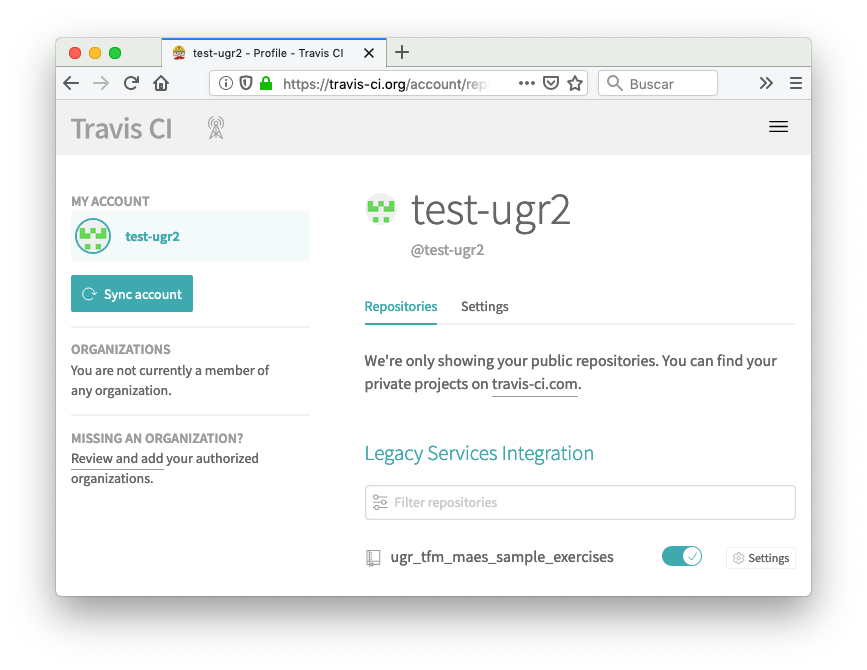
\includegraphics[width=1.0\textwidth]{../images/travis_enable}
\caption{Detalle de activación de un repositorio en Travis CI}
\label{fig:travis_enable}
\end{figure}

Una vez activado, con cada \texttt{git push} se ejecutará el ``pipeline'' definido en el fichero \texttt{.travis.yml}, en nuestro repositorio de ejemplo se puede obtener uno configurado para ejecutar los diferentes ejemplos realizados para mostrar el funcionamiento de la metodología.

\subsection{Introducción a la programación}

Una vez los alumnos han aprendido los comandos básicos de Git y se han dado de alta en GitHub es hora de enseñarles los comandos básicos

\subsubsection{Conceptos básicos de programación}

Todos los lenguajes de programación comparten algunos elementos básicos que funcionan y se usan de forma diferente en cada lenguaje, pero que cumplen el mismo objetivo. Esos elementos son:
Tipos de datos
Variables
Control de flujo
Ciclos
Estructuras de datos
Funciones


\subsubsection{Nuestro primer ``Hola Mundo''}

Un ``Hola mundo'' es un programa cuya única finalidad es escribir la frase ``Hola mundo!''. Este programa se usa como introducción en la mayoría de lenguajes de programación siendo el primer ejercicio típico, y se considera fundamental desde el punto de vista didáctico. Una implementación de dicho programa se puede encontrar para prácticamente todos los lenguajes de programación existentes.

\bigskip
En nuestra metodología animamos a los profesores a enseñar un primer ejemplo del lenguaje a impartir usando un ``Hola Mundo'' para que los alumnos se familiaricen con el lenguaje. En nuestros ejercicios de ejemplo vamos a incorporar el hola mundo como primer ejercicio de programación.

\subsubsection{Guías de estilo}
\subsubsection{Introducción al TDD}
\subsubsection{Algunos ejercicios en diferentes lenguajes}

En el repositorio \url{https://github.com/erseco/ugr_tfm_maes_sample_exercises} hemos definido una serie de ejercicios así como sus correcciones, pasamos a detallar los mismos.


Escribe una función que encuentre el enésimo número primo. Para simplificar, asumimos que la entrada siempre será un entero (int). Si la entrada es menor o igual a 0, la función debe devolver -1.

pasos a seguir para crear un ejercicio

tiempos de creación de ejecución por el alumno

Dichos ejercicios se han incorporado en la sección de Anexos


\subsection{Usando la integración continua para aprender}

Una vez hemos visto como usar Git y los conceptos básicos de programación vamos a ver algunos de los errores con los que se pueden encontrar los alumnos, como pueden usar el sistema de integración continua para detectarlos ellos mismos y como corregirlos.




